\documentclass[]{article}
\usepackage[margin=0.9in]{geometry}

\usepackage{enumitem}
\usepackage{graphicx}
\usepackage{float}
\usepackage{hyperref}
\usepackage[dvipsnames]{xcolor}

% Make it easier to see when we talk about Docks and not Docker
\newcommand{\docks}{\textcolor{Blue}{Docks} }
\newcommand{\docker}{Docker }

% Images in uml/ and user-manual/ have the same names so
% uml/ has not been included here. Instead images/ is included
% so they can be referenced with uml/image.png
\graphicspath{{images/user-manual/}{images/logo/}{images/umlet/}{images/}}

%opening
\title{
	\vspace{-1.5cm}
	
\includegraphics[scale=0.7]{docks_round_512.png}
	\\[1cm]
	Requirements and Design for Docks}
\author{\textbf{Team}: TripleParity\\
\textbf{Client}: Compiax\\
\\
\textbf{Team Members}\\
Francois Mentz\\
Connor Armand du Plooy\\
Raymond De Vos\\
Evert Geldenhuys\\
Anna-Marié Helberg\\
Paul Wood}

\date{}

\begin{document}

\maketitle

\tableofcontents

\pagebreak

\section{System Overview}
\subsection{Purpose}

% Why would I want to use Docks? 
\docker is a tool designed to make it easier to create, deploy and run applications
using lightweight virtualization. It provides a command line interface (CLI)
and RESTful API. Maintaining and deploying applications often involve multiple
people. Providing multiple people access to the \docker CLI requires
Secure Shell access (SSH) as root to the server running \docker. If the server
is secure it will only provide SSH access using public/private keys, which
reduces convenience and restricts access to devices that are SSH capable and
holds a private key. The \docker API lacks functions which are provided by
the CLI, so it cannot be used on its own.

The purpose of \docks is to provide a secure web user interface
for using \docker.

\subsection{Product Scope}

% Cool, you showed the limitations of Docker, now what can Docks do for me?
\docks will provide functionality in three areas
\begin{enumerate}
	\item Provide a secure web user interface that enables using the
	      essential functions exposed by the \docker API and CLI.
	\item Provide a secure API to allow third party services to integrate
	      with \docks and use \docker
	\item Send real time notifications to system administrators via Slack about
	      important events
\end{enumerate}

\subsection{Definitions, acronyms and abbreviations}

% TODO(egeldenhuys): More definitions
\begin{table}[H]
	\begin{tabular}{|p{2cm}|p{10cm}|}
		\hline
		\docks &  A system to provide a web user interface and API for using \docker and managing a \docker swarm \\ \hline

		\docker & Tool designed to make it easier to create, deploy and run applications
		using lightweight virtualization \\ \hline

		Image & ``A container is launched by running an image.
		An image is an executable package that includes everything
		needed to run an application--the code, a runtime, libraries,
		environment variables, and configuration files.'' \\ \hline

		Container & ``A container is a runtime instance 
		of an image--what the image becomes in memory when 
		executed (that is, an image with state, or a user process)'' \\ \hline
		
		Swarm & A tool to schedule and clump docker nodes into a single virtual machine which is easier to use and maintain. \\ \hline
		
		Stack & A group of Docker services that make up an application. \\ \hline
		
		Service & A collection of Docker containers of the same images. \\ \hline
		
		Nodes & Any virtual or physical machines that run Docker and are part of a swarm. \\ \hline

	\end{tabular}
\end{table}

\subsection{UML Domain Model}

\begin{figure}[H]
	\centering
	\includegraphics[scale=0.5]{domain-diagram.png}
	\caption{UML Domain Diagram for the Docks System}
\end{figure}

\section{Functional Requirements}

\subsection{Users}
\docks will appeal mainly to software developers and system administrators
with fundamental understanding of \docker. \docks will allow
them to deploy new applications with \docker as well as manage existing 
applications. With the web user interface they will be able to
update and troubleshoot applications using any web browser. They will
also be able to give access to the web user interface to other administrators
for assisting in management. It is assumed this category of users will
have knowledge on configuring applications to be deployed with \docker
and the ability to troubleshoot networks and applications.

\docks will also appeal to users that are interested in learning how
to use \docker. With \docks they can deploy pre-configured applications and
develop an understanding of the features provided by \docker using the 
web user interface. It is assumed these users know the basic \docker
terminology and can learn from the \docker documentation.

\subsection{Subsystems}
% TODO(egeldenhuys): Make this section easier to read.
% The constant mentioning of Docks API/UI and Docker API makes
% it hard to follow.


% TODO(egeldenhuys): Make component diagram more vertical so that it
% will fit nicer
\begin{figure}[H]
	\centering
	\includegraphics[scale=0.3]{component-diagram.png}
	\caption{Component Diagram for \docks}
\end{figure}

\docks consists of two projects with distinct purposes:
\docks UI which is the web user interface running in the web browser
and \docks API which is the server running on a Manager Node.

\docks UI is responsible for displaying information about applications running
in \docker, and to provide a convenient interface for sending information
to \docker via the \docks API.

\docks API is responsible for providing authenticated access to the \docker API.
It also extends the \docker API by providing the ability to deploy Stacks
and monitor \docker events for sending notifications.

Across these two projects exist a number of subsystems.
Their specific requirements will be enumerator

\subsubsection{Authentication}
The authentication subsystem is responsible for authenticating
and authorizing users as well as managing (create, edit, delete) user accounts.

\begin{figure}[H]
	\centering
	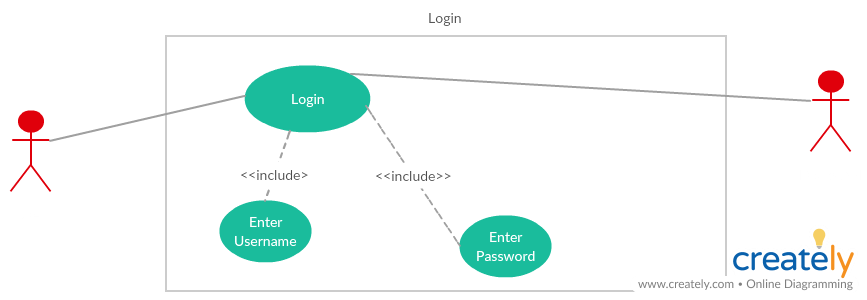
\includegraphics[scale=0.5]{uml/login.png}
	\caption{Use case diagram for Login}
\end{figure}

\subsubsection{WebHooks and Docker Events}
This subsystem is responsible for managing (create, edit, delete) WebHooks.
It interfaces with the Docker API to listen for events and send relevant
data to the stored WebHooks.

\begin{figure}[H]
	\centering
	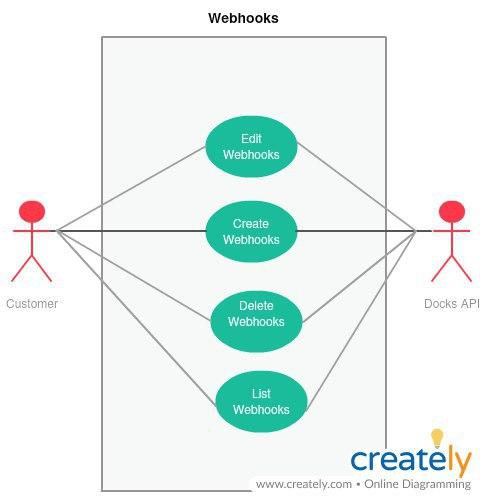
\includegraphics[scale=0.5]{uml/webhooks.png}
	\caption{Use case diagram for WebHooks}
\end{figure}

\subsubsection{Stack API Extension for Docker}
The Stack API Extension for \docker is part of the \docks API.
Since \docker lacks an API for managing Stacks, it has to be implemented
by the \docks API. This will enable \docks UI and third party services
to view and manage \docker stacks.

\begin{figure}[H]
	\centering
	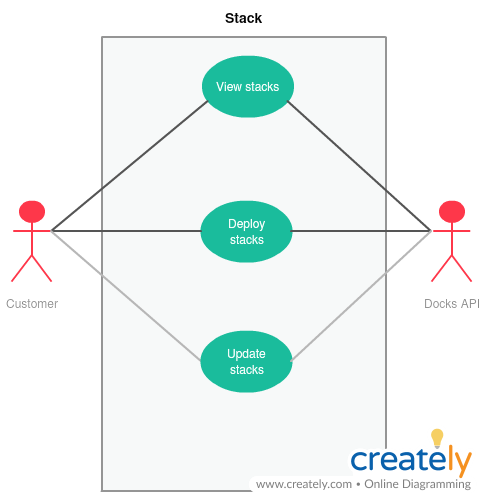
\includegraphics[scale=0.5]{uml/stacks.png}
	\caption{Use case diagram for Stacks}
\end{figure}

\begin{figure}[H]
	\centering
	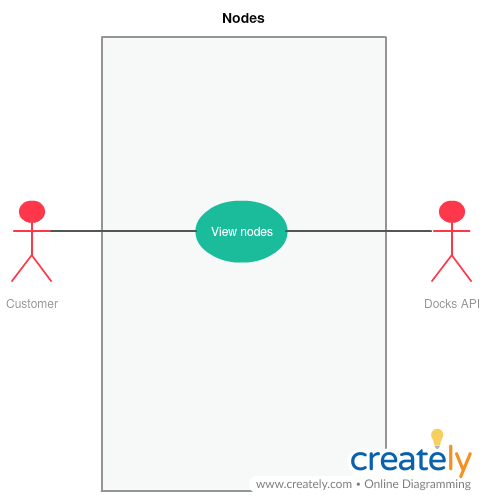
\includegraphics[scale=0.5]{uml/nodes.png}
	\caption{Use case diagram for Nodes}
\end{figure}

\begin{figure}[H]
	\centering
	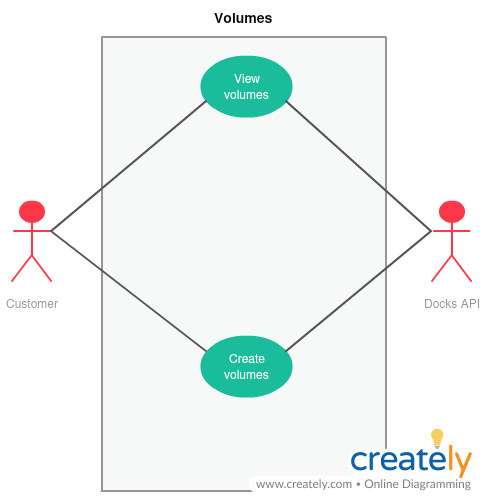
\includegraphics[scale=0.5]{uml/volumes.png}
	\caption{Use case diagram for  Volumes}
\end{figure}

\begin{figure}[H]
	\centering
	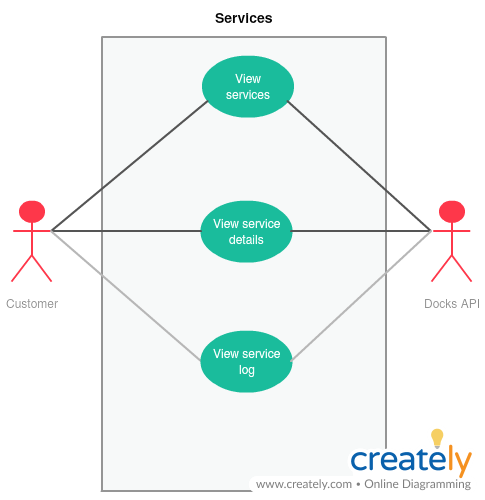
\includegraphics[scale=0.5]{uml/services.png}
	\caption{Use case diagram for  Services}
\end{figure}

\begin{figure}[H]
	\centering
	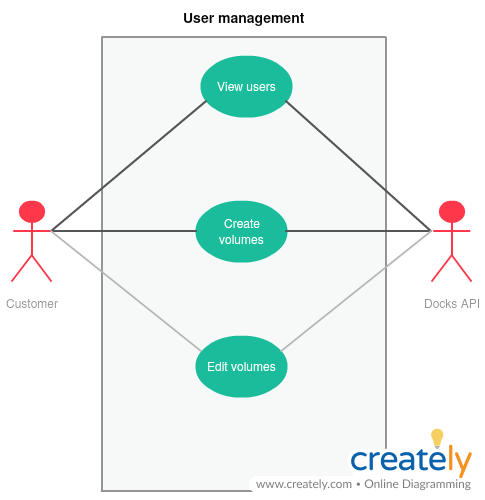
\includegraphics[scale=0.5]{uml/users.png}
	\caption{Use case diagram for  Users}
\end{figure}

\begin{figure}[H]
	\centering
	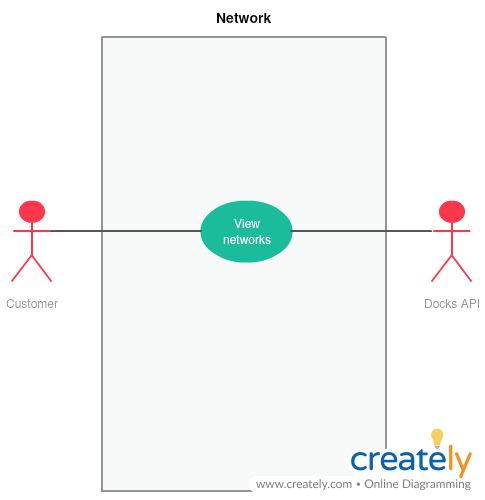
\includegraphics[scale=0.5]{uml/networks.png}
	\caption{Use case diagram for Networks}
\end{figure}

\subsubsection{API Proxy for \docker}
The API proxy 	for \docker is part of the \docks API. It provides authenticated
access to the \docker API through the \docks API. The \docker API is not
exposed directly to the world, rather authenticated users may send
requests to the \docks API to be transparently forwarded to the
private \docker API.

\subsubsection{Frontend \docks API service}
The \docks API service is part of the frontend (\docks UI). It acts as the interface
between the graphical frontend components and the \docks HTTP API.
This layer of abstraction means that the network logic is hidden from
components that need to interact with the \docks API.

\subsubsection{\docker Management Functions}
\docker will be managed from the \docks UI, through the authenticated
\docks API. The user should be able to perform common operations
from \docks UI such as deploying an application and viewing its state.

\subsection{Specific Requirements}

\subsubsection{WebHooks and Docker Events}
\begin{enumerate}[label=R1.\arabic*.]
	\item The system shall allow a user to add new outgoing WebHooks
	\item The system shall display a list of added WebHooks
	\item The system shall allow a user to remove a WebHook
	\item The system shall allow a user to specify the type of events to send to the WebHook
	\item The system shall monitor all \docker events and send the relevant event data to the respective WebHook
	\item The system shall send a Slack notification to WebHooks that should receive node events
\end{enumerate}

\subsubsection{Authentication}
\begin{enumerate}[label*=R2.\arabic*.]
	\item The system shall allow an authorized user to interact with the Docks API
	\item The system shall provide the ability to use two factor authentication as described in RFC 6238
	\item The system shall provide a global administrative account role without restrictions
	\item The system shall provide the following user management features to be used by administrative accounts
	\begin{enumerate}[label*=\arabic*.]
		\item Create new administrative user
		\item Remove user
		\item Update user password
		\item Enable and disable two factor authentication
	\end{enumerate}
\end{enumerate}

\begin{figure}[H]
	\centering
	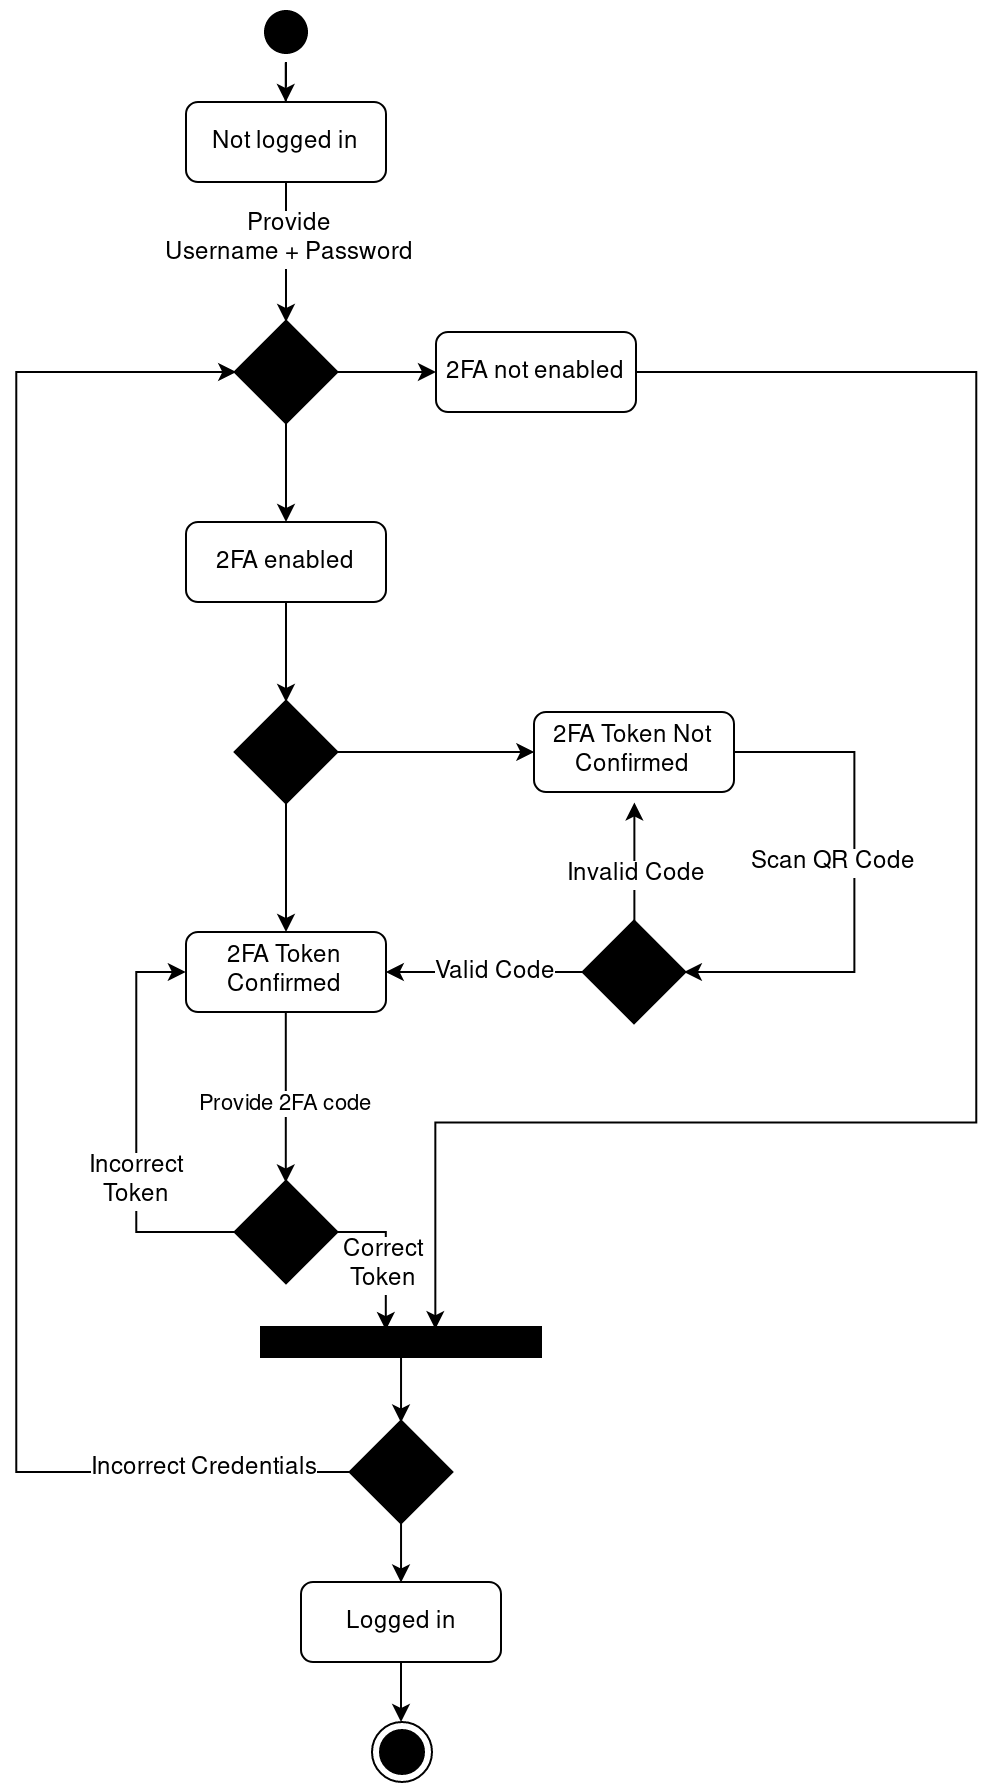
\includegraphics[width=\textwidth,height=\textheight,keepaspectratio]{uml/login-state-diagram.png}
	\caption{State diagram for user authentication}
\end{figure}

\subsubsection{Stack API Extension for Docker}
\begin{enumerate}[label*=R3.\arabic*.]
	\item The system shall provide the ability to deploy new stacks given the stack name and docker-compose file
	\item The system shall provide the ability to return deployed stacks along with the number of services in each stack
	\item The system shall provide the ability to update a stack
	\item The system shall provide the ability to remove a stack
	\item The system shall not allow a stack to be created if it already exists
	\item The system shall not allow a stack to be updated if it does not exist
	\item The system shall provide the ability to return the services that are part of a given stack
\end{enumerate}

\subsubsection{API proxy for Docker}
\begin{enumerate}[label*=R4.\arabic*]
	\item The system shall only forward requests to the \docker API if the request was made by an authenticated user
	\item The system shall not modify content forwarded from the \docker API to the user
	\item The system shall not modify requests forwarded from the user to the \docker API
	\item The system shall forward error messages from the \docker API to the user
\end{enumerate}

\subsubsection{Docker Management Functions}
\begin{enumerate}[label*=R5.\arabic*.]
	\item The system shall display all nodes
	\item The system shall display all stacks
	\item The system shall display all services
	\item The system shall display all tasks
	\item The system shall display all networks
	\item The system shall display all volumes
	\item The system shall allow a user to upload a docker-compose file to deploy a Stack
	\item The system shall allow a user to remove a stack from the swarm
	\item The system shall display the tasks that are running in a service
	\item The system shall allow a user to view the log of a service
	\item The system shall allow a user to update a stack using a docker-compose file
	\item The system shall allow a user to delete a volume
	\item The system shall allow a user to delete a network
\end{enumerate}

\subsubsection{Frontend \docks API service}
\begin{enumerate}[label*=R6.\arabic*.]
	\item The system shall provide the interface for all requirements stated in the "Docker Management Functions" section above
	\item The system shall provide meaningful error message to the user
\end{enumerate}

\section{Non-functional Requirements}
\subsection{Quality}
Quality requirements entail the reliability and availability of the system. Both are important for our system because Docks allows a company to manage their whole Docker Swarm. In other words, the system must be available so that one can manage the Swarm (and reliabilty for the same reason). 

This will be achieved by having Docks runcompletely offline. Docker also allows you to specify what happens when a service goes down within its respective compose file, for example, to restart the service or kill the service completely.Docks run as a service that is set up to restart on failure which means that Docks will be available most of the time.

To test whether the requirements are met, one can test the uptime but as we run Docks via Docker the reliabilty and availablity are taken of by Docker itself.

\subsection{Safety}
Safety involves the ability to prevent the system from entering an unwanted state because of an unintended operation. This is important because because if the system enters an unwanted state it can affect the availability or reliability of the system. 

Docks implement path guards to protect the system when a wrong path is entered. It will simply return a 404 error. Docks also implement a confirmation system for all of the actions that can be performed to ensure that accidental deletions or updates are not made to critical services. For example, user input is validated for stacks to prevent them from overriding existing data.

The metric to test the paths can be using Fuzzing. This technique generates different urls within Docks' scope and outputs data such as whether incorrect urls were accepted or correct urls were rejected. The metric for testing whether input is correct would be to apply user testing.

\subsection{Security}
Security entails protecting the system resources. This is done by authenitcation and different types of users. 

Authentication is achieved by two-factor authenication (which involves scanning a QR Code with your phone) and by using a token-based approach. Not all users have the same privileges in the system and the type is assigned once a user registers and can be updated by the administrator.

Docks applies npm-audit which performs a security review of the system and tell you about the vulnerabilities within your dependencies and how to fix them. User testing can also be performed to verify authentication.

\section{System}
\subsection{Interfaces}
\subsubsection{Software Interfaces}
Since the frontend cannot securely interface with the Docker API,
an intermediate interface will be developed (Docks API).
The Docks API will communicate between the frontend (Docks-UI) and
the Docker API. The Docks API will provide a simplified interface for
interacting with the Docker API.


\subsection{System Configuration}
The Deployment diagram shows the architecture from the device perspective.

\begin{figure}[H]
	\centering
	\includegraphics[scale=0.5]{deployment-diagram.png}
	\caption{UML Deployment Diagram for the Docks System}
\end{figure}

\subsection{Architectural Styles}
% TODO: Clarify this section

The User Interface uses the Model View Controller architecture.
Nodes and Containers have a data model.
The user interacts with the view to manipulate the data model.
The view is updated when the data model retrieves data using an N-Tier architecture.
The 3-Tier architecture can be seen by the actor interacting with the view,
the request is then delegated to the models, which in turn
communicate with other objects to retrieve and set the required data from
the Docker API server and Docker Swarm.

\begin{figure}[h]
	\centering
	\includegraphics[scale=0.4]{architecture-diagram.png}
	\caption{MVC and 3-Tier Architecture diagram for the Docks system}
\end{figure}


\end{document}
